\vspace{-4pt}
\section{Preliminary}
\vspace{-4pt}
In this section, we will first formulate the automated agentic workflows generation problem in Section~\ref{sub:problem} and then discuss design considerations of our \model in Section~\ref{sub:design}. For the core concept of this section, we provide an example explanation in Figure~\ref{formulation}.

\begin{figure}[t!]
  \centering
  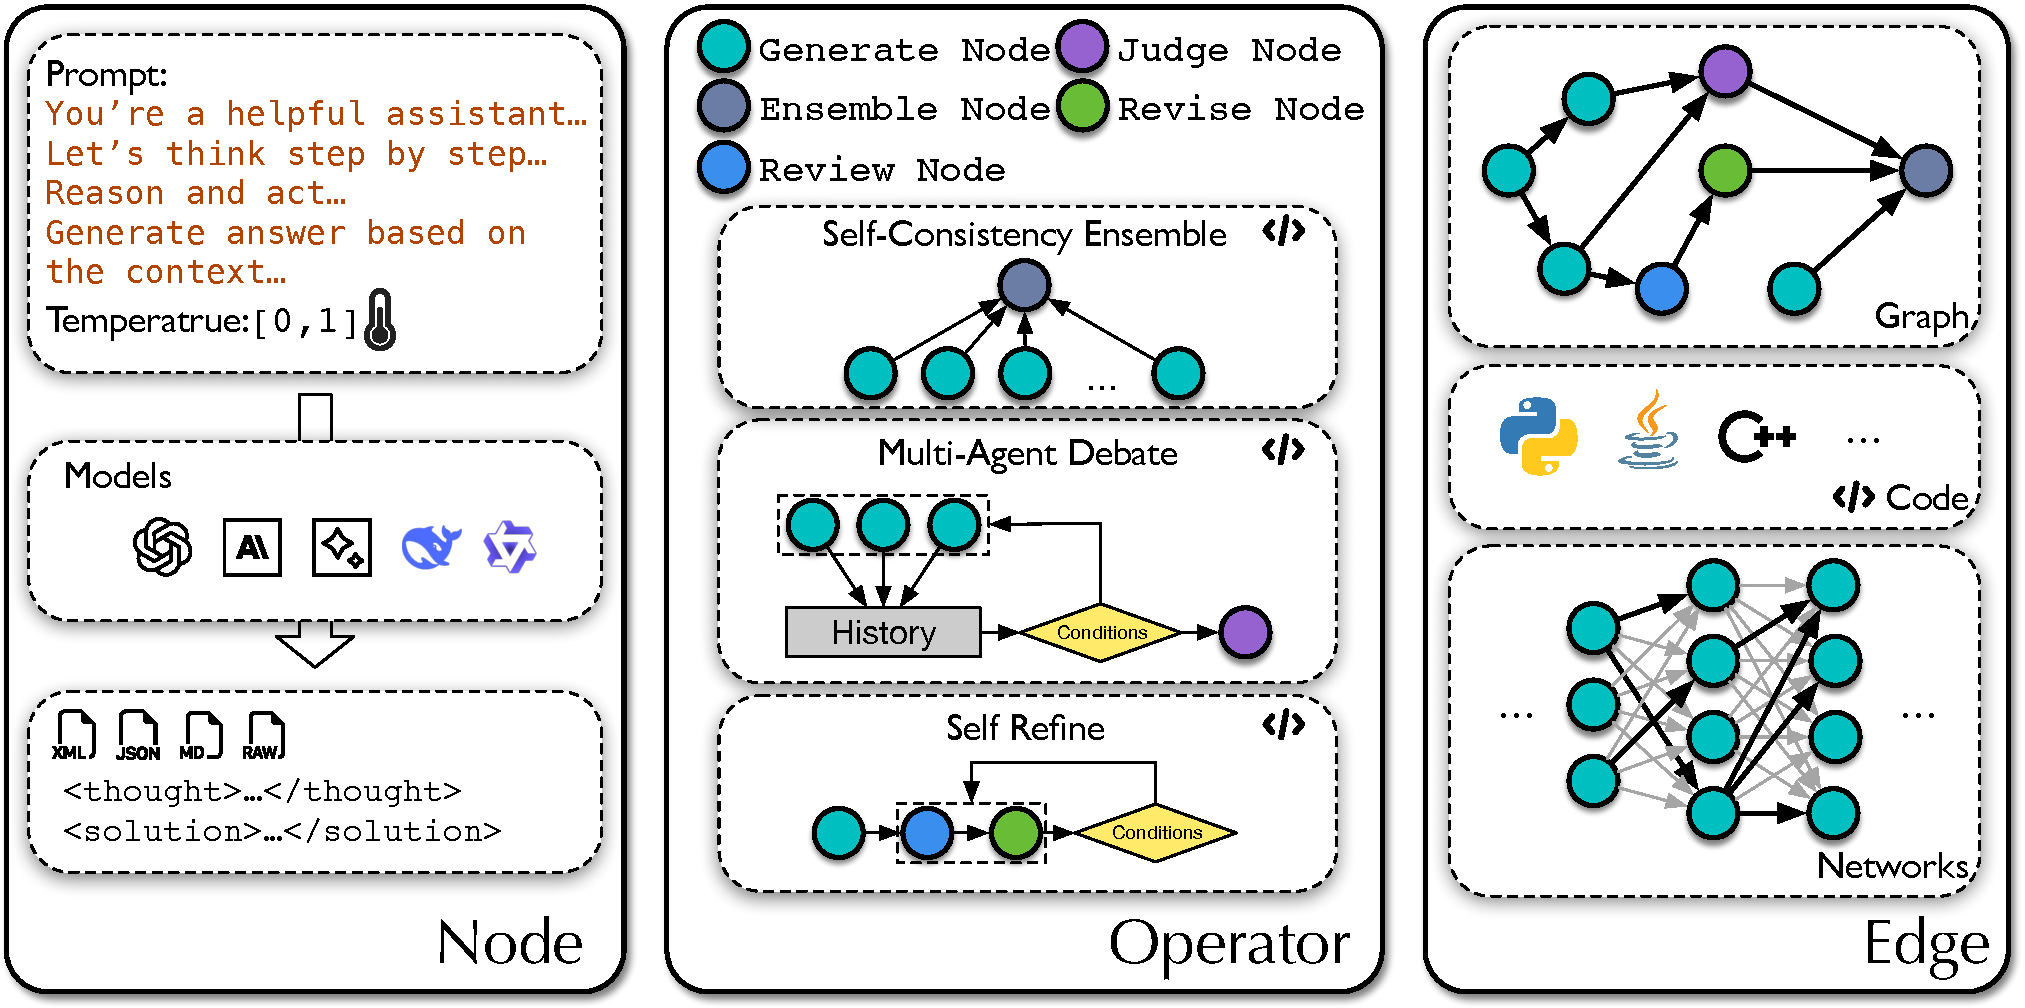
\includegraphics[width=\linewidth]{images/FORMULATION.pdf}
  \vspace{-7mm}
  \caption{\textbf{The example of node, operator, and edge.} We demonstrate the optional parameters for Nodes, the structure of some Operators, and common representations of Edges.}
  \label{formulation}
  \vspace{-3mm}
\end{figure}

\subsection{Problem Formulation} 
\label{sub:problem}

\paragraph{Agentic Workflow}
\label{para:workflow}
We define an agentic workflow W as a series of LLM-invoking nodes connected by edges to define the exection orders, denoted as \( \mathcal{N} = \{ N_1, N_2, \ldots, N_i \ldots \} \). Each node \( N_i \) represents a specific operation performed by an LLM and is characterized by the following parameters. The code abstraction of the node is shown in Appendix \ref{appendix:node structure}.
{
\begin{itemize}[leftmargin=20pt]
    \item \textbf{Model \( M \)}: The specific language model invoked at node \( N_i \).
    \item \textbf{Prompt \( P \)}: The input or task description provided to the model at each node.
    \item \textbf{Temperature \( \tau \)}: A parameter controlling the randomness of the LLM’s output at node \( N_i \).
    \item \textbf{Output format \( F \)}: The format in which the model's output is structured (\textit{e.g.}, xml, json, markdown, raw). The node in workflow should provide different output formats, inspired by the ~\citet{zhi2024format}.
    
\end{itemize}
}

Edge \( E \) represent abstract structures defining node relationships, governing the sequence of execution. The edge \( E \) can be represented via various structures, such as:

\begin{itemize}[leftmargin=20pt]
    \item \textbf{Graph ~\cite{zhuge2024gptswarm}}: A flexible structure representing hierarchical, sequential, or parallel relationships between nodes, allowing for complex branching workflows.
    \item \textbf{Neural Network ~\citep{liu2023dynamic}}: A structure that can represent complex, non-linear relationships between nodes, allowing for adaptive and learnable workflows based on input and feedback.
    \item \textbf{Code ~\citep{hu2024automated}}: A comprehensive representation that can express linear sequences, conditional logic, loops, and incorporate graph or network structures, offering the most precise control over workflow execution for LLMs.
\end{itemize}

While graph structures can represent workflow relationships, they require complex extensions (e.g., Petri nets, BPMN) beyond basic DAGs to naturally express parallel execution and conditional logic. Neural networks enable adaptive transitions but lack precise control over workflow execution. In contrast, code representation inherently supports all these relationships through standard programming constructs. Therefore, we adopt code as our primary edge structure to maximize expressivity.

\paragraph{Automated Workflow Optimization}
Given a task \( T \) and an evaluation function \( G \), the goal of workflow optimization is to discover a workflow \( W \) that maximizes \( G(W, T) \). This can be formulated as a search process where an algorithm \( A \) explores the search space \( \mathcal{S} \) to determine the optimal workflow configuration.
The search space \( \mathcal{S} \) for a workflow optimization problem encompasses all possible configurations of node parameters and edge structures:

\[
\mathcal{S} = \{ (\mathcal{N}, E) \mid  E \in \mathcal{E} \},
\]

where \( \mathcal{N} = \{ N(M, \tau, P, F) \mid M \in \mathcal{M}, \tau \in [0,1], P \in \mathcal{P}, F \in \mathcal{F} \} \), with \( \mathcal{M}, \mathcal{P}, \mathcal{F}, \mathcal{E} \) representing the sets of possible language models, prompts, output formats, and edge configurations, respectively.

With this formulation, the workflow optimization problem can be expressed as:

\[
\begin{aligned}
W &= A(\mathcal{S}, G, T), \\
W^* &= \argmax_{W \in \mathcal{S}} G(W, T),
\end{aligned}
\]

where \( A \) is the search algorithm that explores the search space \( \mathcal{S} \), and \( W^* \) is the optimal workflow configuration that maximizes the evaluation function \( G \) for the given task \( T \).

% \subsection{Preliminary}
\subsection{\model Overview}
\label{sub:design}

\paragraph{Limitations of Previous Methods}
Previous approaches ~\cite{mert2024text, omar2024dspy, zhuge2024gptswarm} to workflow optimization have primarily been constrained by the limited scope of their search spaces, based on problem definition in Section~\ref{sub:problem}. Another related work, ADAS~\citep{hu2024automated}, searches in a larger space comprising a combination of prompts $N(P, T)$ and edges $E$, but fails to discover effective workflows due to the efficiency limitations of its linear heuristic search algorithm.


\begin{figure}[t!]
  \centering
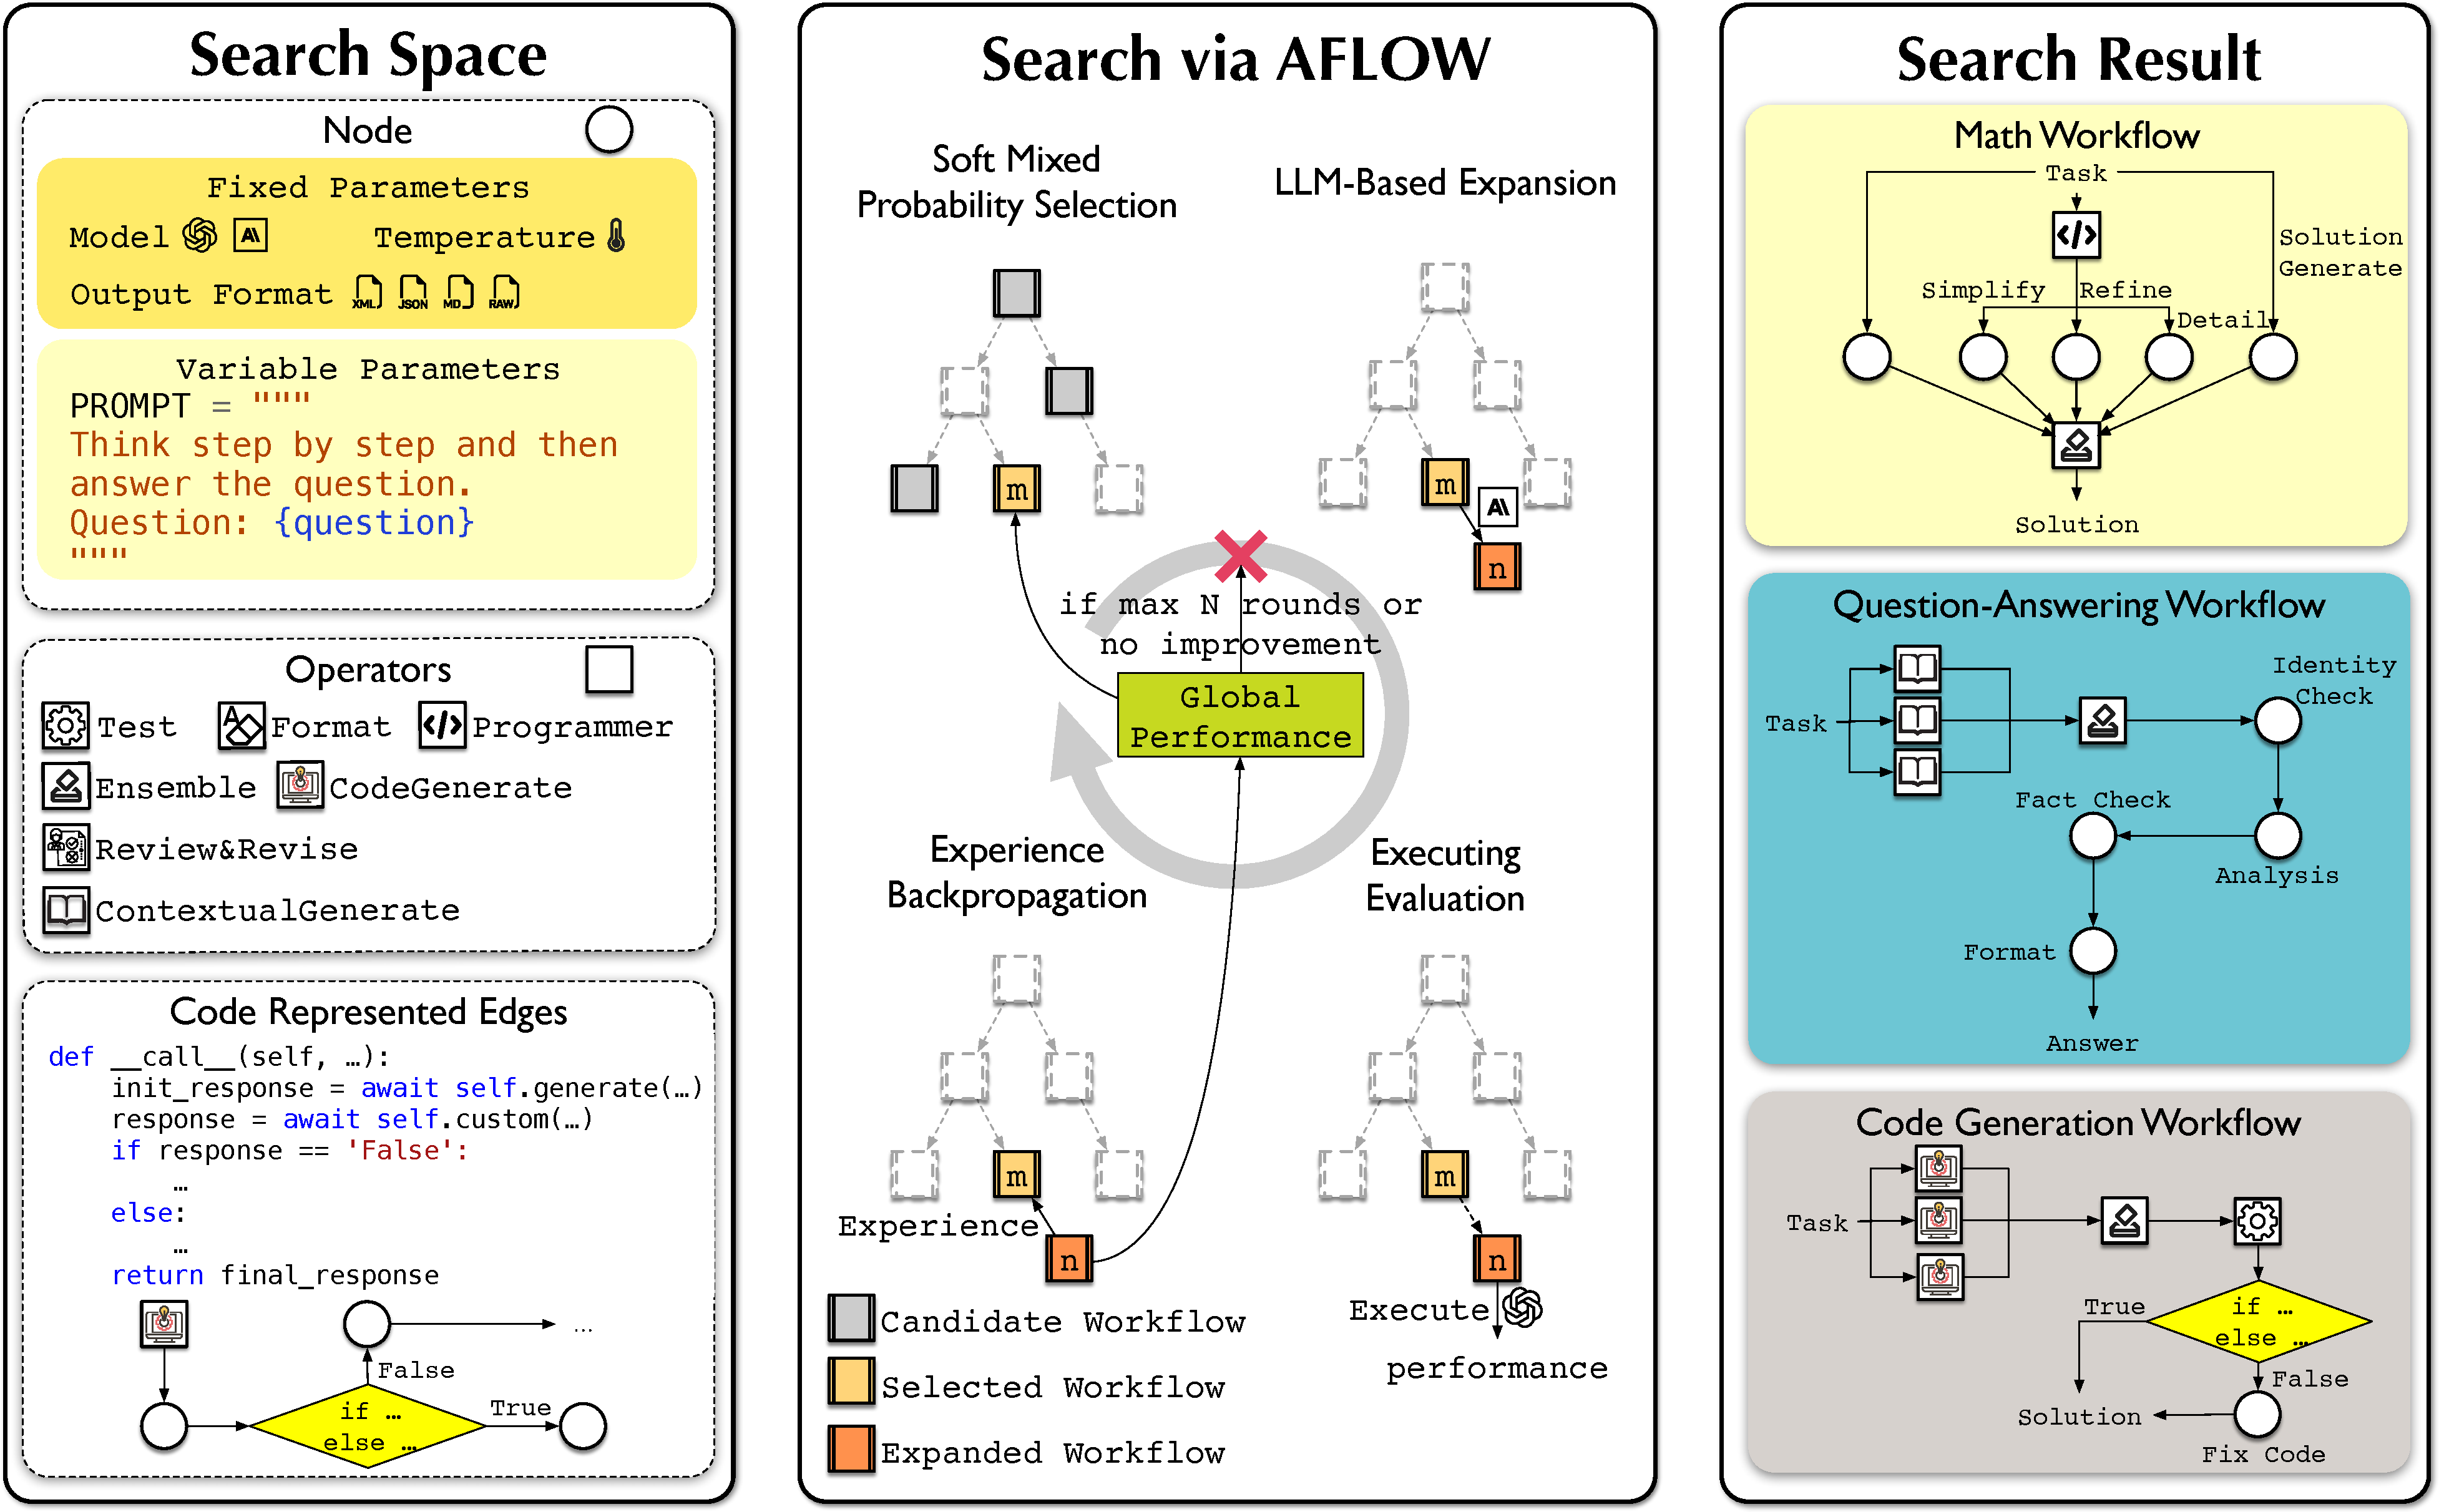
\includegraphics[width=\linewidth]{images/MCTS.pdf}
 \vspace{-7mm}
  \caption{\textbf{Overall \modelbold framework}: By setting a search space composed of nodes with only prompt parameters flexible, a given operator set, and a code representing edge, \model performs an MCTS-based search within this space. Through a variant of MCTS designed for workflow optimization, \model iteratively executes a cycle of Soft Mixed Probability Selection, LLM-Based Expansion, Execution Evaluation, and Experience Backpropagation until reaching the maximum number of iterations or meeting convergence criteria.}
  \label{mcts}
  \vspace{-3mm}
\end{figure}

\paragraph{Formulation}
To address the limitations of previous methods, we propose \model, a novel framework that leverages Large Language Models (LLMs) as optimizers within a variant of Monte Carlo Tree Search (MCTS) to search for optimal workflows. 
As discussed in Section \ref{para:workflow}, edges can be represented in both graphs and code. To ensure AFLOW can explore the full range of possible agentic workflows, we represent nodes N and edges E through code.
Specifically, as shown in Figure~\ref{mcts}, \model uses a variant of MCTS to iteratively explore the workflow search space, evaluate different configurations, and backpropagate experiences to refine the workflow optimization process.
% By representing nodes $N$ and edge $E$ through code, 
% \model can explore the full range of possible agentic workflows, ensuring completeness in the search space.


To enhance search efficiency in practice, we simplify the search space by fixing key parameters such as the model $M$, temperature $\tau$, and format $F$. This simplification allows \model to focus its search primarily on the code-represented edges $E$ and prompts. To navigate this still vast search space effectively, we introduce the concept of \textbf{Operators}. These Operators encapsulate common agentic operations (e.g., Ensemble, Review, Revise) by combining $N$ and $E$ into unified interfaces, thereby enabling more efficient utilization by \model. By employing these Operators, we achieve more efficient search and streamlined workflow generation.

Formally, given a set of Operators $\mathcal{O}$ that represents predefined node combinations, and an edge space $\mathcal{E}$ represented through code, the optimization problem can be formalized as:

\begin{equation}
\mathcal{S}_\text{AFlow} = \{ (P_1, \ldots, P_n, E, O_1, \ldots, O_n) \mid P_i \in \mathcal{P}, E \in \mathcal{E}, O_i \in \mathcal{O} \} \\
\end{equation}
\begin{equation}
W^* = \text{\model}(\mathcal{S}_\text{AFlow}, G, T) 
\end{equation}

\paragraph{Tasks Scope and Operations}
% In this paper, we focus on applying \model to reasoning tasks with numerical evaluation functions. 
% We extract common operations from existing literature and define them as part of the operator set~$\mathcal{O}$.
 % These operations include:
% (1) Generate, (2) Format, (3) Review and Revise \cite{madaan2023self},
% (4) Ensemble \cite{wang2022COTSC}, 
% (5) Test \cite{li2024debug}, and (6) Programmer. The operator set $\mathcal{O}$ can be easily expanded to enhance search efficiency for various tasks. Alternatively, \model can perform searches with an empty Operator Set, offering flexibility in implementation. The efficiency comparison between these approaches is detailed in Section~\ref{sec:ablation}. For a comprehensive understanding of the operators, we provide their detailed structures in Appendix~\ref{appendix:operator_code}. 

In this paper, we focus on applying \model to reasoning tasks with numerical evaluation functions. We extract common operations from existing literature and define them as part of the operator set~$\mathcal{O}$.
These operations include:
(1) Generate, (2) Format, (3) Review and Revise \cite{madaan2023self},
(4) Ensemble \cite{wang2022COTSC},
(5) Test \cite{li2024debug}, (6) Programmer, and (7) Custom as the default operator for basic node construction. The operator set $\mathcal{O}$ can be easily expanded to enhance search efficiency for various tasks. Even without any predefined operators, \model can construct different workflow nodes using the basic Custom operator. The efficiency comparison between these approaches is detailed in Section~\ref{sec:ablation}. For a comprehensive understanding of the operators, we provide their detailed structures in Appendix~\ref{appendix:operator_code}.

\section{The Design Details of \model} 
The core concept of \model is to employ Large Language Models (LLMs) as optimizers within a Monte Carlo Tree Search (MCTS) variant to discover effective workflows. In our MCTS structure, \textbf{each tree node represents a complete workflow rather than individual LLM-invoking node}, enabling the discovery of universal solutions for classes of problems. The search process operates through an iterative cycle of soft mixed probability selection, LLM-based optimization expansion, execution evaluation, and experience backpropagation until reaching maximum iterations or convergence criteria. A simplified illustration is shown in Figure \ref{mcts}, with detailed algorithm process and theoretical analysis presented in Appendix \ref{appendix:algorithmaflow} and Appendix \ref{appendix:theroy}, respectively.

Existing workflow optimization methods iteratively use past workflow structures to prompt LLMs to discover new structures. However, due to information loss during accumulation (as input tokens increase), this approach struggles to guide LLMs towards specific performance metrics. Combined with the vast search space of code, this reduces search efficiency.
Our \textbf{key idea} is to leverage the tree structure of MCTS to preserve workflow-based exploration experiences in $N_{max}$ rounds workflow optimization. When a workflow is revisited, we accurately reuse past successful experiences and avoid failures, enabling effective workflow generation and improving search efficiency. To prevent local optima, we introduce a special selection mechanism allowing generation from a blank template at any round.
Next, we will introduce the complete process of \model, as shown in Algorithm \ref{alg:concise-mcts-workflow-optimization}.


\begin{algorithm}[!t]
\caption{Algorithm of \model: Detailed implementation}
\label{alg:concise-mcts-workflow-optimization}
\begin{algorithmic}[1]
\Require Evaluator $G$, Dataset $D$, Operators $\mathcal{O}$
\Ensure Optimized Workflow $W^*$

\State Initialize $W_0$, split $D$ into $D_V$ and $D_T$
\State $W^* \gets W_0$

\For{$iteration \gets 1$ to $N_{max}$}
    \State $workflow \gets$ Select(tree) \Comment{Using soft mixed probability strategy}
    \State $child.workflow \gets$ Expand($workflow$, $\mathcal{O}$) \Comment{LLM-based expansion}
    \State $score \gets$ Evaluate($child.workflow$, $G$, $D_V$) \Comment{Multiple runs for robustness}
    \State Backpropagate($child.workflow$, $score$) \Comment{Update experience and scores}
    \State Update $W^*$ if improved
    \If{ConvergenceCriteriaMet()}
        \textbf{break}
    \EndIf
\EndFor

\State \Return $W^*$
\end{algorithmic}
\end{algorithm}

\textbf{Initialization}
\model begins with a template workflow $W_0$, which provides a framework for invoking nodes and operators. The code template, detailed in Appendix \ref{appendix:graph structure}, allows the LLM optimizer to complete workflow simply by completing call functions. Prior to initiating the search process, we randomly partition the dataset into a validation set (20\%) and a test set (80\%), with the random seed fixed at 42. To optimize computational efficiency, \model then executes the blank template five times on the validation dataset. From these executions, we select a subset of problems that exhibit high variance in scores, which becomes the final validation set.

\textbf{Selection}
Our algorithm forms the initial workflow by evaluating an empty workflow on the validation set. And then continuously select workflows based on a soft mixed probability selection strategy. 
c% 
We propose this strategy for workflow optimization: combining uniform and score-based weighted probability distributions to select from top-k workflows and the initial workflow, where including the initial workflow ensures persistent exploration capability while avoiding local optima. The formula for this selection strategy is as follows:

\begin{equation}
P_{\text{mixed}}(i) = \lambda \cdot \frac{1}{n} + (1 - \lambda) \cdot \frac{\exp(\alpha \cdot (s_i - s_{\text{max}}))}{\sum_{j=1}^{n} \exp(\alpha \cdot (s_j - s_{\text{max}}))},
\end{equation}

\vspace{-2pt}

$\text{where } n \text{ is the number of workflows}, s_i \text{ is workflow } i \text{'s score}, s_{\text{max}} \text{ is the maximum score}, \alpha \text{ }(0.4) \\ \text{ controls } 
\text{score influence, and } \lambda \text{ }(0.2) \text{ balances exploration and exploitation}.$

\textbf{Expansion}
In the expansion phase, we employ an LLM as an optimizer to create new workflows and the optimize prompt is illustrated in Appendix \ref{appendix:prompt}. The optimizer leverages the selected workflow's experience to generate new prompts or modify node connections by altering code, resulting in new workflows. Specifically, to maximally uncover insights from past iterations, the experience includes all modifications and their corresponding improvements or failures on the selected workflow, along with precise logs of predictions and expected output.

\textbf{Evaluation}
\model directly executes workflows to get feedback due to explicit evaluation functions in reasoning tasks. We test each generated workflow 5 times on the validation set, computing mean and standard deviation. While this increases per-iteration cost, it provides more accurate feedback for the optimizer. This precision enhances search efficiency, ultimately reducing the number of iterations required to reach an effective solution.

\textbf{Backpropagation}
After execution, we record: (1) the workflow's performance, (2) the optimizer's modification of its parent workflow, and (3) optimization success relative to its parent. This information is stored in experience and propagated back to the parent workflow, while the performance score is added to the global record for selection.

\textbf{Terminal Condition}
We implement early stopping to reduce unnecessary execution costs: the process terminates if the top-k average score shows no improvement for $n$ consecutive rounds, or after $N$ total rounds otherwise. See Appendix \ref{appendix:algorithmaflow} for algorithmic details.
